\documentclass[10pt,a4paper,twocolumn]{article}

\usepackage[T1]{fontenc}
\usepackage[utf8]{inputenc}

\usepackage[english]{babel}
\usepackage{natbib}
\usepackage{url}

\usepackage{subfigure}

\usepackage{graphicx, grffile}
\graphicspath{{../assets/}}

\usepackage{booktabs}

\title{Personal Reflections: Some thoughts on writing}
\author{Nazarov Ivan}

\begin{document}
\maketitle

I, personally, find the following guidelines and methods useful and productive for
writing text and pouring thoughts onto digital medium. They may be naive or silly, but
it think it is worth documenting them here. By the way this text itself may not follow
them by the letter, but hopefully does not gravely violate them.

Below is a brief recollection of what urged me to compose this scribble in early
Autumn of 2019:
\begin{quote}
  I used to follow them, but then lost my way due to stress and personal issues and
  forgot what it feels to actually `Feel` these principles. Luckily, such us the human
  nature, that one Wednesday evening, feeling particularly down from the paper that
  dragged on and on, I decided to force myself into not putting fragments, but complete
  thoughts into the text. I began a new document and pushed myself into getting a hold
  of my scattered ideas about composing text, they once again dawned onto me. I seem
  to have rebounded.
\end{quote}

Anyway, below are the guidelines, that strive for one goal: writing better quality
narrative in my academic/personal texts (not that many have been written so far, though).

\section{Avoid sentence/thought fragments} % (fold)
\label{sec:avoid_sentence_thought_fragments}

As soon as possible and not later, but always coalesce fragments into complete sentences
and/or coherent text fragments.

The train of thought is orders of magnitude faster than typing. Thus it is permitted
to write sentences/text out of order, skipping ahead to compose the ending or key phrases,
and backtracking afterwards to fill in the gaps. Place the pieces where ever they seem
to be relevant or belong in the tentative plan of the text.

Try to formulate what you want to write (at least crudely and partially) before actually
writing -- some planning and thought does ignite the mind and put you in the "flow".
It is not forbidden to type and design a sentence in Russian (native language), before
actually translating it to English.

% section avoid_sentence_thought_fragments (end)

\section{Fractal text structuring} % (fold)
\label{sec:fractal_text_structuring}

The overall narrative follows the classic structure: from general to specific. We introduce
something, develop it, draw conclusions, and move on either by getting more specific, or
shifting focus onto the connected topic or related concept. Focus on a single idea within
a paragraph, section, plot, or table.

Paragraph contains one complete piece of thought and its structure is the same: intro-%
main-outro, -- with cohesive devices interspersed here and there to string them together.
Paragraphs themselves exist within this narration flow: some paragraphs introduce, other
relay ideas concepts and the rest summarize or draw conclusion from the narrative in the
former.

% section fractal_text_structuring (end)

\section{The text is malleable material} % (fold)
\label{sec:the_text_is_malleable_material}

Writing text can benefit from programming styles and techniques. Adopt modular hierarchical
treatment of sentences, paragraphs, and sections. Top-down writing style works wonders:
begin with coarse plan, then progressively refine its element and ultimately being
coalescing the letters into words into phrases, into sentences, into paragraphs and
sections.

Always try to come up with synonyms when writing sentences -- this increases variety,
and broadens the perspective.

% section the_text_is_malleable_material (end)

\section{Iterative process} % (fold)
\label{sec:iterative_process}

Writing text is an iterative process of constant addition, removal, refinement and
revision. Just like research: submit for feedback, update, then rinse and repeat.

\begin{figure}
  \centering
  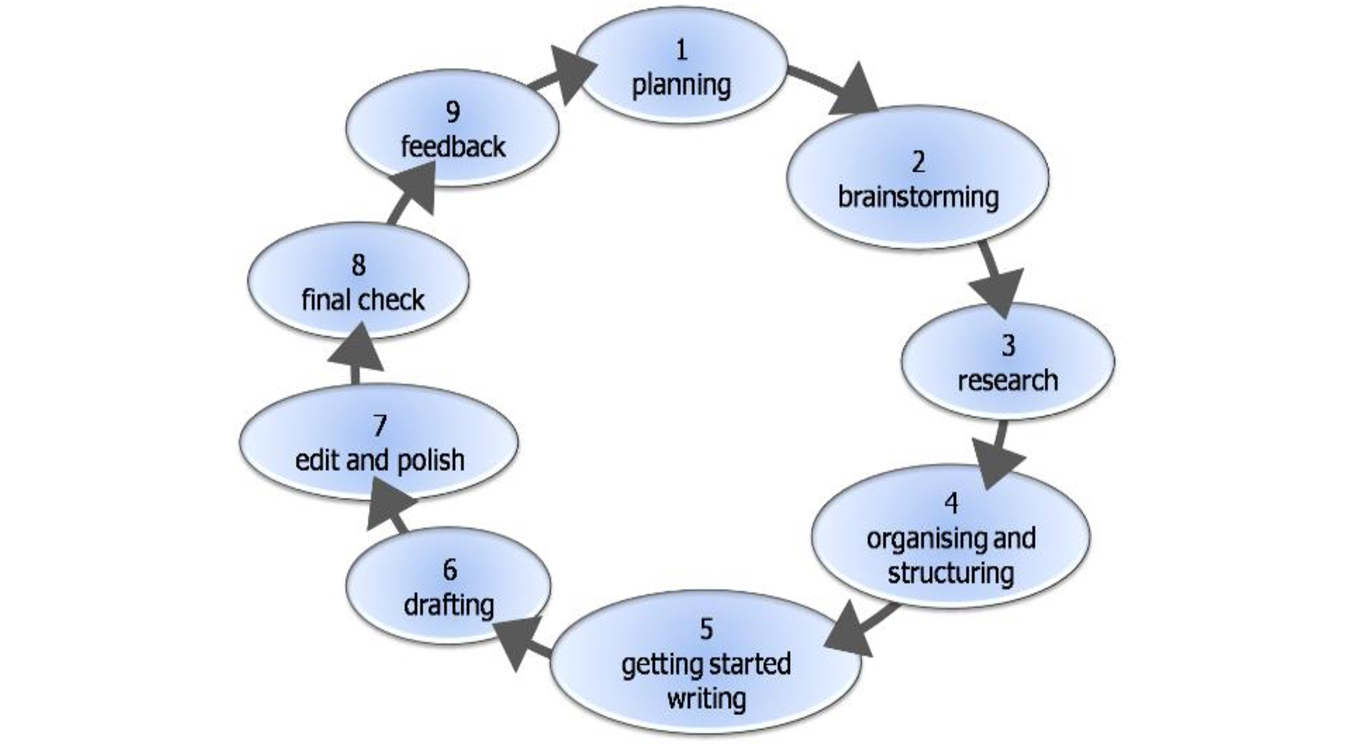
\includegraphics[width=\columnwidth]{assets/iterative_process.pdf}
  \caption{
    The cyclic process of writing.
  }
\end{figure}

% section iterative_process (end)

\section{General narrative guidelines} % (fold)
\label{sec:general_narrative_guidelines}

The following rules are mostly listed as imperatives.

Don't include things (text, sentence, ideas) that are not your point. Do not add a formula
just for the sake of a formula. The narrative must flow: introduce concepts before using
them, refer to them as necessary, or even reproduce their condensed versions when needed.
Connect and develop ideas within text: what is the focus now builds upon what came before.
Try to keep related things close to each other -- that way it requires much less cognitive
load to understand the main idea of the paragraph, section or text.

% section general_narrative_guidelines (end)

\section{Writing and research} % (fold)
\label{sec:writing_and_research}

% some general words
Research is finding answers to questions using appropriate methods (fig.~\ref{fig:direction}).
It is an process of systematic analysis of available information and prior findings
aimed at providing insight and conclusions. The process is aimed at testing carefully
formulated hypotheses and proposals using methods designed or selected with due care
and attention. Ultimately research relates to the synthesis of new actionable in broad
sense knowledge, based on the existing theory, past findings and original insight.

Research is carried out with the intent of making relevant contribution to the field. It
relies on organized and closely analysed materials, including prior art, which informs
its own direction and focus. The focus is put in the context of the current state of its
discipline: relevant theoretical basis, recurrent issues and topics, historic and current
debates, various perspectives and significant contributions.
\begin{figure}
  \centering
  \begin{subfigure}
    \centering
    \includegraphics[width=\columnwidth]{assets/direction.png}
  \end{subfigure}%
  \begin{subfigure}
    \centering
    \includegraphics[width=\columnwidth]{assets/research_context.png}
  \end{subfigure}
  \caption{
    Obvious in hindsight.
  }
  \label{fig:direction}
\end{figure}

The core part of the research is its written account, which details the process, hypotheses,
and methods, brings out significance of the findings (``so what?''), spells out implications
and conclusions. The write up demonstrates the progression of the chain of research findings
and critically evaluates the findings in context.

% lit review and context
The context of the research in the write up is contained in the literature review, related
work, and discussion sections. They help build the narrative by providing coverage and
analysis of the relevant knowledge base, significant prior research and key issues. In the
course of the narrative the context is interpolated onto the present findings, is drawn
upon for comparison, criticism, explanation or support. Context is built on broad reading,
is aware of a wide range or related work, yet remains focused on carefully curated prior
research and specialized papers, their contributions and limitations.

% As an integral part of research activity, writing is not done after everything is carried out.
Writing must be an integral part of research activity, not a step done after the experiments.
In science you start with a hypothesis, test it then toss it out -- all of this reflected
in text. Text is dispensable: each writing activity is useful, but do not cling to text,
code or any other literary expression.

Having many drafts is normal and encouraged: each draft must be checked for assumptions,
terminology, logical correctness.

A seemingly good advice is to try writing an early draft of the conclusion, which might
give a solid sense of direction, and used as a reminder of the research hypothesis. Since
the findings are written up on-the-go, this draft will inevitably be updated to reflect the
recent developments, contradictory or refuting evidence.

% getting started and managing
Like every project, research requires advanced resource management skills: work process
organization and planning, self-management, time management, scheduling, and risk assessment.

% reword this
When setting out to research a new topic, it is important to develop a sense of the method
needed to arrive at the expected answer to the posed question in the ``end product''. Having
this understanding will help make task scheduling easier and manageable.
%
Begin by diligently surveying the field, focusing reading and thinking on potential topics,
and formulate research questions and hypotheses. Then think how you will answer the question
or test the hypothesis and develop a detailed overview of the basic process, considering
potential complexities.
%
Then prepare the materials, fine-tuning thinking, research question and methods. Start project
planning process, detailing tasks and steps and making sense of what they entail. Identify and
clarify steps and work out the best order. But don't dive right in, orient yourself with the
task from start to finish. Always keep accurate and coherent records of what you do, organize
your to-do lists and logs, set writing targets.

% section writing_and_research (end)

\end{document}
